\documentclass [a4paper,final,conference,10pt]{IDAACS}
\usepackage[utf8]{inputenc}
\usepackage[english]{babel}
\usepackage{amsmath}
\usepackage{graphicx}
\usepackage{multirow}
\usepackage{cite}

%\title{Effective Parallelization of Mixed-Critical Software to Distributed Heterogeneous Mutlicoresystems}
%\subtitle{
%	Approaching Challenges of Automotive Constrains: Partial Realtime, Safety, Affinity and Connectivity}
%Bare-Metal and OS-based 
%\title{Constrained Parallelization of Mixed-Critical Applications to Distributed Heterogeneous Hardware}
\title{Constrained Mixed-Critical Parallelization for Distributed Heterogeneous Systems}

\author{
\IEEEauthorblockN{Robert Höttger\IEEEauthorrefmark{1}, Mustafa Özcelikörs\IEEEauthorrefmark{1}}
%						Third Author's Name\IEEEauthorrefmark{2}}

\IEEEauthorblockA{\IEEEauthorrefmark{1}Dortmund University of Applied Sciences and Arts - IDiAL Institute, \\\{robert.hoettger, mustafa.ozcelikors\}@fh-dortmund.de, www.idial.org\\
%						\IEEEauthorrefmark{2}Affiliation, Postal address, e-mail, Web address (URL)\\
%						\IEEEauthorrefmark{3}Affiliation, Postal address, e-mail, Web address (URL)\\
	}
}

\begin{document}
\maketitle

\let\thefootnote\relax\footnotetext{As part of the AMALTHEA4public project, this work has been funded by the German Federal Ministry of Education and Research - BMBF, under funding no. $01|S14029K$}

\begin{abstract}
Distributing software effectively to multi-core, many-core, and distributed systems has been studied for decades and still advances successively driven by domain specific constraints. Programming vehicle ECUs (Electronic Constrol Units) is one of the most constrained domains that just recently approached the need for concurrency due to advanced driver assistant systems or autonomous driving approaches. In this paper, various challenges for such systems are outlined, discussed, and solutions are given upon instruction precise modeling, affinity constrained based distribution, and effective software parallelization. The solutions are compared upon bare-metal and OS based implementations while considering fixed priorities for sequential, OS based, and APP4MC scheduling. The latter case has been published at \cite{ICPDSSE} and evolved to consider affinity constraints, SWC-based partitioning and communication cost related mapping. Results show that using APP4MC based distributions on a distributed heterogeneous system outperforms available approaches for mixed-critical applications. %TODO percent

\end{abstract}

\begin{IEEEkeywords}
component; formatting; style; styling
\end{IEEEkeywords}

\section{Introduction}

Especially the automotive domain requires lots of constraints originating from different safety, security, timing, or similar requirements. The verification, validation, testing, and simulation stack requires dozens of tools and the consideration of established architectures, standards, models, and assessments to address product-line supporting, consistent, modular, and scalable software. However, these efforts lack in transparency likewise the comprehensive understanding of applications. Recent approaches \ref{APP4MC} already address this challenge and try to provide a common adaptable platform based on AUTOSAR while providing a standardized data model. Any specific commercial or proprietary tooling is supposed to be integratable in order to provide seamless interaction with provided tooling such as product-line management, requirements engineering, partitioning, mapping, testing, and more. 

In this paper, use the open source APP4MC environment in order to address both industrial and research related models while evaluating our new developments not only regarding model results but also to validate result among a specific use case described in section \ref{sec:rccar}. The RC-Car is an advanced demonstrator that features 16 100MHz cores (XMOS ExplorerKit, XCore 200) 
%2 instructions per cycle see https://www.xmos.com/download/private/xCORE-Architecture-Flyer%281.1%29.pdf
%2000MIPS 16 core https://www.xmos.com/download/private/xCORE-200-XE-Product-Brief%281.2%29.pdf

combined with four cores clocked at 1200MHz (Raspberry Pi 3, ARM CoreTex-A53).
The further remainder of this paper is structured as follows: The next section \ref{sec:app4mc} describes roughly the environment this contribution is based upon. Afterwards, section \ref{sec:rccar} illustrates capabilities and properties of the RC-Car demonstrator. Subsequently, section \ref{sec:impl} outlines the specific developments and solutions to precise modeling and software parallelization that is evaluated and compared to related approaches in section \ref{sec:eval}. Finally, section \ref{sec:concl} concludes this paper's contributions and discusses benefits, disadvantages, possible extensions, and promising outlooks that potentially advance the current approach.


\section{APP4MC}
\label{sec:app4mc}

\section{RC-Car}
\label{sec:rccar}
The current Raspberry Pi distribution includes processes for the touchscreen, ethernet communication, core utilization reader, mjpg streamer, vnc application, apache2, OpenCV image processing, and additional cyclewaster. The latter processes can be added in order to push the core utilization to a maximum and consider high workload. The effective distribution provided by APP4MC is here crucial to provide deadline violation free program execution. 

The XMOS tasks are implemented on a more precise level and focus on necessary real time implementations. Scheduling on the XMOS is non preemptive and allows a better determinism as well as easier WCET reasoning due to less context switching and less scheduling jitter \ref{xmos}. However, since our number of tasks exceed the total number of available cores on the XMOS, we had to define high priority tasks, that run on a dedicated core, and low priority tasks that run concurrently with other low level tasks in cooperative multitask fashion on common cores. The amount of high priority tasks thereby defines the number of cores available for the low priority tasks. 
%EQUATION-----------------------------------------------
%\begin{equation}
%\label{Eq_1}
%\lambda_i = \lim \frac{1}{p} \sum_{t=1}^p \ln \frac{|w_i (t)|}{|w_i (t-1)|}
%\end{equation}

\section{Precise modeling and Software Parallelization}
\label{sec:impl}

%FIGURE-----------------------------------------------
%\begin{figure}[bth]
%\centering
%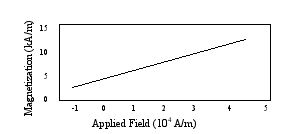
\includegraphics[scale=0.6]{images/Fig1.png}
%\caption{\label{Fig_Magnet}Magnetization as a function of applied field. Note 
%how the caption is centered in the column.}
%\end{figure}

%TABLE-----------------------------------------------
%\begin{table}[htb]
%\caption{Table Type Styles}
%\label{Table_I}
%\centering
%\begin{tabular}{|p{1.2cm}|p{1.5cm}|p{1.5cm}|p{1.5cm}|}
%\hline
%\multirow{2}{1.2cm}{\textbf{Type Size (pts.)}} & \multicolumn{3}{|c|}{\textbf{Appearance}}\\
%\cline{2-4}
% & \textbf{\textit{Regular}}&\textbf{\textit{Bold}}&\textbf{\textit{Italic}}\\
%\hline
%8 & References, table header, footnotes, text subscripts, and superscripts &&\\
%\hline
%\end{tabular}
%\end{table}

\section{Evaluation and Related Work}
\label{sec:eval}

\section{Conclusion}
\label{sec:concl}

\section*{Acknowledgment}
The authors would like to express their appreciation to ...
\enlargethispage{-7in}

\bibliographystyle{IEEEtran}
\bibliography{IEEEabrv,IDAACS_Example}
\end{document}